\documentclass[12pt]{article}

\usepackage{sbc-template}
\usepackage{graphicx,url}
\usepackage[utf8]{inputenc}
\usepackage[T1]{fontenc}
\usepackage{amsmath,amssymb,amsfonts}
\usepackage{booktabs}
\usepackage{float}
\usepackage{microtype}

\renewcommand{\refname}{Referências}
\renewcommand{\figurename}{Figura}
\renewcommand{\tablename}{Tabela}

\urlstyle{same}
\sloppy
\raggedbottom

\renewenvironment{abstract}{%
  \vspace{6pt}\begin{center}\normalfont\bfseries Abstract\end{center}\nopagebreak
  \list{}{\leftmargin=1cm\rightmargin=\leftmargin
          \listparindent=1.27cm\itemindent=\listparindent}%
  \item[]\normalfont\small}%
  {\endlist\vspace{4pt}}
\renewenvironment{resumo}{%
  \vspace{6pt}\begin{center}\normalfont\bfseries Resumo\end{center}\nopagebreak
  \list{}{\leftmargin=1cm\rightmargin=\leftmargin
          \listparindent=1.27cm\itemindent=\listparindent}%
  \item[]\normalfont\small}%
  {\endlist\vspace{4pt}}

\title{Topologia da Malha Metroferroviária de São Paulo:\\
  uma Análise via Teoria dos Grafos}

\author{Vitor Eduardo Silva de Carvalho\inst{1}, Diego Naoki Sato Hanashiro\inst{1},\\
  João Vitor Ribeiro Pereira\inst{1}, Joaquim Argolo Valente de Azambuja\inst{1}}

\address{Bacharelado em Ciência e Tecnologia (BC\&T)\\
  Universidade Federal do ABC (UFABC)\\
  Av. dos Estados, 5001 -- 09210-580 -- Santo André -- SP -- Brasil
  \email{\shortstack{\{vitor.eduardo, diego.hanashiro\}@aluno.ufabc.edu.br\\
      \{joao.pereira, joaquim.azambuja\}@aluno.ufabc.edu.br}}
}

\begin{document}

\thispagestyle{empty}
\vspace*{-0.6cm}

\begin{center}
  \noindent\rule{\textwidth}{1pt}\\[12pt]
  {\LARGE\bfseries Topologia da Malha Metroferroviária de São Paulo:\\[4pt]
   uma Análise via Teoria dos Grafos\par}
  \vspace{12pt}
  \noindent\rule{\textwidth}{3pt}
\end{center}

\vspace{16pt}

\begin{center}
  \begin{minipage}[t]{0.32\textwidth}\centering
    \textbf{Vitor Eduardo Silva de Carvalho}\\[4pt]
    {\footnotesize vitor.eduardo@aluno.ufabc.edu.br}
  \end{minipage}\hfill
  \begin{minipage}[t]{0.32\textwidth}\centering
    \textbf{Diego Naoki Sato Hanashiro}\\[4pt]
    {\footnotesize diego.hanashiro@aluno.ufabc.edu.br}
  \end{minipage}\hfill
  \begin{minipage}[t]{0.32\textwidth}\centering
    \textbf{João Vitor Ribeiro Pereira}\\[4pt]
    {\footnotesize joao.pereira@aluno.ufabc.edu.br}
  \end{minipage}

  \vspace{12pt}

  \begin{minipage}[t]{0.45\textwidth}\centering
    \textbf{Joaquim Argolo Valente de Azambuja}\\[4pt]
    {\footnotesize joaquim.azambuja@aluno.ufabc.edu.br}
  \end{minipage}
\end{center}

\vspace{6pt}
{\centering\footnotesize
  Bacharelado em Ciência e Tecnologia (BC\&T) --- Universidade Federal do ABC (UFABC)\\
  Av.\ dos Estados, 5001 --- 09210-580 --- Santo André --- SP --- Brasil\par}

\vspace{12pt}

\begin{abstract}
  We model the metropolitan rail network of São Paulo as a graph (stations are
  vertices; track segments between consecutive stations are edges) and
  characterize its topology --- degree, global efficiency, clustering,
  centrality, community structure and small-world indices --- assessing
  robustness under random failures and targeted attacks. The network proves
  sparse and strongly radial: it is \emph{neither} scale-free \emph{nor} a small
  world in space-L ($\sigma=0.43$), is dominated by the Luz and Brás hubs, and
  collapses under targeted attacks. Modeled identically, London and New York are
  denser and more redundant. We also quantify the new Line 6-Orange and show that
  an orbital line would improve connectivity far more than new radial ones.
\end{abstract}

\begin{resumo}
  Modelamos a malha metroferroviária de São Paulo como um grafo (estações são
  vértices; trechos entre estações consecutivas são arestas) e caracterizamos sua
  topologia --- grau, eficiência global, agrupamento, centralidade, comunidades e
  índices de mundo pequeno ---, avaliando a robustez sob falhas aleatórias e
  ataques dirigidos. A rede mostra-se esparsa e fortemente radial: \emph{não} é
  livre de escala \emph{nem} de mundo pequeno no espaço L ($\sigma=0{,}43$), é
  dominada pelos \emph{hubs} Luz e Brás e colapsa sob ataques. Modeladas do mesmo
  modo, Londres e Nova York são mais densas e redundantes. Quantificamos ainda a
  Linha 6-Laranja e mostramos que uma linha orbital ajudaria muito mais que novos
  raios.
\end{resumo}

% =====================================================================
\section{Introdução}
% =====================================================================

Sistemas de transporte de massa são redes complexas: estações ligadas por
trechos de via cujo arranjo global determina eficiência, vulnerabilidade e
capacidade de reorganização~\cite{newman2003}. A teoria dos grafos revelou que
metrôs de cidades muito distintas compartilham assinaturas estruturais ---
caráter de mundo pequeno, poucos \emph{hubs} de alta centralidade e distribuições
de grau de cauda longa~\cite{latora2002,sen2003,derrible2010}.

A Região Metropolitana de São Paulo possui a maior rede sobre trilhos do Brasil:
em meados de 2026, com a Linha 6-Laranja, a malha integrada (Metrô e CPTM) soma
cerca de $393$~km, $15$ linhas e $182$ estações~\cite{metrosp2026,cptm2026}.
Apesar da escala, ela raramente é estudada sob a ótica formal de grafos. Este
trabalho tem por \textbf{objetivos}: (i) modelar a malha como grafo e
caracterizar sua topologia; (ii) identificar as estações estruturalmente
críticas e medir a robustez da rede; (iii) comparar São Paulo com Londres e Nova
York sob a mesma metodologia; e (iv) avaliar o impacto da Linha 6 e de linhas
futuras. As Seções seguintes trazem a fundamentação, o problema, os dados, os
resultados, a discussão, as considerações finais e a divisão de tarefas.

% =====================================================================
\section{Definições e Fundamentação Teórica}
% =====================================================================

Modelamos a rede como um grafo simples, não direcionado e conexo $G=(V,E)$, com
$N=|V|$ estações e $M=|E|$ arestas. Na representação em \emph{espaço L}
\cite{vonferber2009}, existe aresta $\{i,j\}$ se as estações são consecutivas em
alguma linha; a matriz de adjacência é $A=[a_{ij}]$. Uma estação de baldeação,
servida por várias linhas, é \emph{um} único vértice de grau maior. Na
representação em \emph{espaço P}, duas estações são adjacentes se pertencem à
mesma linha, e a distância conta \emph{baldeações} --- adequada à experiência do
usuário.

O grau $k_i=\sum_j a_{ij}$ tem média $\langle k\rangle = 2M/N$. Terminais têm
$k_i=1$, estações intermediárias $k_i=2$ e baldeações $k_i\geq 3$. Seja $d(i,j)$
o menor caminho entre $i$ e $j$; o comprimento característico é
$L=\tfrac{1}{N(N-1)}\sum_{i\neq j} d(i,j)$ e o diâmetro $D=\max_{i,j} d(i,j)$. Como
$d$ diverge sob desconexão, usa-se a \emph{eficiência global}~\cite{latora2001}:
\begin{equation}
  E_{\mathrm{glob}}(G)=\frac{1}{N(N-1)}\sum_{i\neq j}\frac{1}{d(i,j)}.
\end{equation}
O coeficiente de agrupamento médio $C$ mede a fração de vizinhos de um vértice
que também são vizinhos entre si. Uma rede é de \emph{mundo pequeno}
\cite{watts1998} quando tem $L$ próximo ao de um grafo aleatório equivalente e
$C$ muito maior, medido por $\sigma=(C/C_{\mathrm{rand}})/(L/L_{\mathrm{rand}})$,
com $\sigma>1$ indicando o comportamento. \emph{Mundo pequeno} (alto $C$, baixo
$L$) não deve ser confundido com \emph{livre de escala}~\cite{barabasi1999}, que
se define pela presença de \emph{hubs} e cauda longa em $P(k)$: são propriedades
independentes. Aqui, ``\emph{hub}'' designa apenas estação de alto grau/
centralidade, não evidência de rede livre de escala.

A criticidade de uma estação é medida pela centralidade de
intermediação~\cite{freeman1977},
$C_B(v)=\sum_{s\neq v\neq t}\sigma_{st}(v)/\sigma_{st}$, onde $\sigma_{st}$ é o
número de caminhos mínimos entre $s$ e $t$ e $\sigma_{st}(v)$ os que passam por
$v$; e pela proximidade $C_C(v)=(N-1)/\sum_j d(v,j)$. Comunidades (grupos mais
densamente ligados internamente) são detectadas maximizando a
modularidade~\cite{newman2006} $Q$ pelo método de Louvain~\cite{blondel2008}. A
robustez é avaliada pela fração $S(f)$ da maior componente após remover uma
fração $f$ das estações, comparando remoção \emph{aleatória} (falha) e
\emph{dirigida} aos vértices mais centrais (ataque)~\cite{berche2009}; usa-se
ainda o índice de Derrible e Kennedy~\cite{derrible2010} $r_T=\mu/N$, com
$\mu=M-N+1$ o número de ciclos independentes (rotas alternativas).

% =====================================================================
\section{Descrição do Problema}
% =====================================================================

Buscamos caracterizar a topologia da malha e suas vulnerabilidades, respondendo:
(1) \textbf{Centralidade:} quais estações concentram os caminhos mínimos? A
hipótese é que baldeações do centro expandido (Sé, Luz, Brás) dominem. (2)
\textbf{Mundo pequeno:} a rede exibe os índices típicos de outros metrôs? (3)
\textbf{Robustez:} quão sensível é a conectividade à perda de poucas estações, e
qual a diferença entre falhas e ataques? (4) \textbf{Comunidades:} a partição de
modularidade máxima tem significado geográfico? Trata-se de um problema de porte
médio ($N\sim 10^2$), tratável de forma exata por algoritmos polinomiais.

% =====================================================================
\section{Dados e Modelagem}
\label{sec:dados}
% =====================================================================

Os dados provêm do mapa oficial da rede da RMSP~\cite{metrosp2026,cptm2026},
considerando as linhas de Metrô (1-Azul, 2-Verde, 3-Vermelha, 4-Amarela,
5-Lilás, 6-Laranja, 15-Prata, 17-Ouro) e de trens metropolitanos (7-Rubi a
13-Jade). Para cada linha extrai-se a sequência ordenada de estações; da Linha 6,
recém-inaugurada, considera-se o trecho em operação (João Paulo I--Perdizes),
ligado à malha pela baldeação em Água Branca.

O grafo em espaço L é construído assim: cada estação distinta é um vértice
(identificado por nome canônico) e, para cada linha
$(s_1,\dots,s_{n})$, adicionam-se arestas $\{s_p,s_{p+1}\}$ entre estações
consecutivas. Vértices são \emph{estações}; arestas são \emph{trechos de via}
diretos; na versão não ponderada $w_{ij}=1$ (opcionalmente, distância ou tempo).
Estações de baldeação acumulam arestas de várias linhas, tornando-se pontos de
articulação. As métricas são calculadas com a biblioteca
NetworkX~\cite{hagberg2008}; código, dados e instruções de reprodução estão em
\url{https://github.com/VitorCarvalho67/GrafosMetroSP}.

% =====================================================================
\section{Resultados}
% =====================================================================

\paragraph{Estrutura (Q1--Q2).} A malha é conexa, com $N=182$, $M=196$ e
$\langle k\rangle=2{,}15$ (Tabela~\ref{tab:metricas}). O grau máximo é $6$ (Luz)
e $79\%$ das estações têm grau $2$: não há cauda longa, logo a rede \emph{não} é
livre de escala. O comprimento característico é alto ($L=13{,}5$; $D=34$) e a
eficiência global $E_{\mathrm{glob}}=0{,}112$. Comparando a $300$ grafos
aleatórios, $C\approx C_{\mathrm{rand}}$ mas $L\gg L_{\mathrm{rand}}$, dando
$\sigma=0{,}43<1$: no espaço L a rede \emph{não} é de mundo pequeno. Essa
propriedade só surge no espaço P ($L_P=2{,}57$, $D_P=5$; $\approx 1{,}6$ baldeação
entre estações quaisquer), que reflete a experiência de viagem.

\begin{table}[ht]
  \centering
  \caption{Índices estruturais da malha de São Paulo.}
  \label{tab:metricas}
  \small
  \begin{tabular}{@{}lr lr@{}}
    \toprule
    Estações $N$ & 182 & Agrupamento $C$ & 0{,}009 \\
    Trechos $M$ & 196 & Mundo pequeno $\sigma$ & 0{,}43 \\
    Grau médio $\langle k\rangle$ & 2{,}15 & Modularidade $Q$ & 0{,}815 \\
    Compr.\ caract.\ $L$ & 13{,}47 & Comunidades & 14 \\
    Diâmetro $D$ & 34 & Robustez $r_T$ & 0{,}082 \\
    Eficiência $E_{\mathrm{glob}}$ & 0{,}112 & Baldeações & 24 \\
    \bottomrule
  \end{tabular}
\end{table}

\paragraph{Hubs (Q1).} As estações de maior intermediação
(Figura~\ref{fig:hubs}) são Luz ($C_B=0{,}47$) e Brás ($0{,}46$), seguidas de
Tatuapé, Lapa, Tamanduateí e Barra Funda --- os complexos de baldeação do centro
expandido, confirmando a hipótese. Estações de grau $2$ com alta intermediação
(Juventus-Mooca, Ipiranga) são pontos de articulação da Linha 10 cuja remoção
isola ramais.

\begin{figure}[ht]
  \centering
  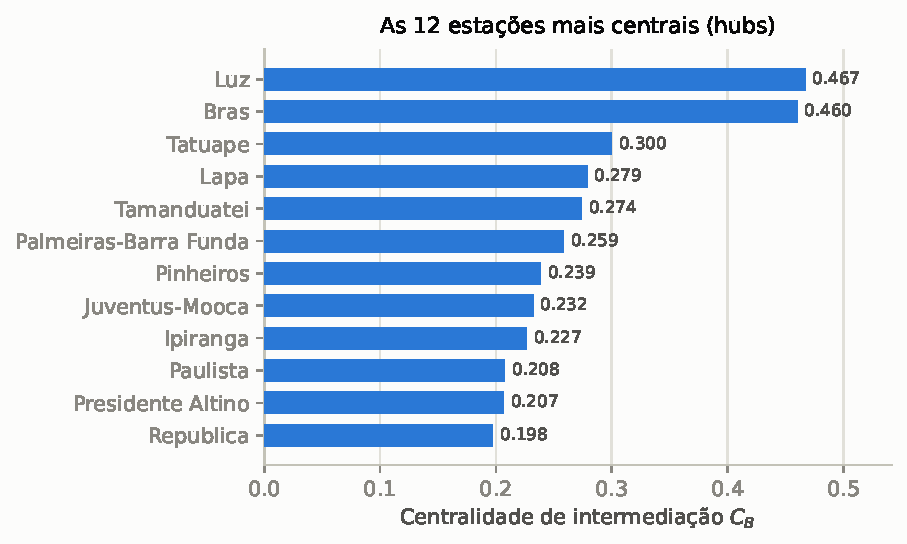
\includegraphics[width=0.72\textwidth]{fig_hubs.pdf}
  \caption{As doze estações de maior centralidade de intermediação.}
  \label{fig:hubs}
\end{figure}

\paragraph{Comunidades e regiões (Q4).} Louvain recupera $14$ comunidades com
$Q=0{,}815$ (alto, típico de redes em corredores), com claro sentido geográfico.
Usando a proximidade média como acessibilidade regional, o centro expandido
(Luz, Brás, República, Barra Funda; $\overline{C_C}=0{,}109$) é cerca de
\emph{duas vezes} mais acessível que as comunidades periféricas
($\overline{C_C}\approx 0{,}06$): a eficiência não é homogênea no território.

\paragraph{Robustez (Q3).} Sob falha aleatória a degradação é gradual (a $10\%$
removido, a maior componente ainda tem $56\%$); sob ataque dirigido o colapso é
abrupto --- bastam $2\%$ das estações (Luz, Brás, Tatuapé, Lapa) para cair a
$57\%$, e $4\%$ para $19\%$ (Figura~\ref{fig:robustez}). A robustez integrada é
$0{,}15$ (falha) contra $0{,}04$ (ataque). A rede resiste a falhas difusas mas é
muito vulnerável à perda de poucos \emph{hubs} centrais.

\begin{figure}[ht]
  \centering
  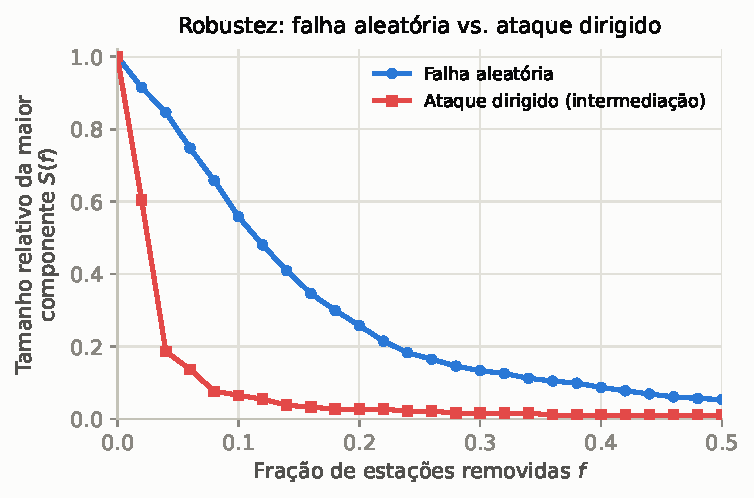
\includegraphics[width=0.72\textwidth]{fig_robustez.pdf}
  \caption{Robustez $S(f)$: falha aleatória vs.\ ataque dirigido por
    intermediação.}
  \label{fig:robustez}
\end{figure}

\paragraph{Comparação com Londres e Nova York.} Modelamos o \emph{London
Underground} e o \emph{New York City Subway} do mesmo modo, a partir dos mapas
oficiais~\cite{tfl2024,mta2024} (Tabela~\ref{tab:tres}). Nossos $r_T$ calculados
coincidem com os publicados por Derrible e Kennedy~\cite{derrible2010} para São
Paulo ($0{,}082$ vs.\ $0{,}080$) e Londres ($0{,}143$ vs.\ $0{,}140$), validando
o método; Nova York, modelada por \emph{serviços} (linhas que compartilham
trilhos), tem $r_T$ superestimado. O contraste-chave está no mundo pequeno: São
Paulo é a \emph{única} das três com $\sigma<1$; Londres ($1{,}86$) e Nova York
($3{,}14$) o cruzam, com o dobro/triplo do agrupamento (Figura~\ref{fig:ind3}).
São Paulo é, de longe, a mais esparsa, radial e menos redundante --- ao lado de
Berlim entre os metrôs menos malhados do mundo, e distante de Paris e
Tóquio~\cite{derrible2010}.

\begin{table}[ht]
  \centering
  \caption{Comparação direta (mesma \emph{pipeline}). $^\ast$Nova York modelada
    por serviços, o que infla baldeações e $r_T$ (valor de linha
    publicado: $0{,}088$~\cite{derrible2010}).}
  \label{tab:tres}
  \small
  \begin{tabular}{@{}lrrrrrr@{}}
    \toprule
    & $N$ & $\langle k\rangle$ & $C$ & $\sigma$ & Baldeações & $r_T$ \\
    \midrule
    São Paulo & 182 & 2{,}15 & 0{,}009 & \textbf{0{,}43} & 0{,}132 & 0{,}082 \\
    Londres   & 258 & 2{,}28 & 0{,}022 & 1{,}86 & 0{,}236 & 0{,}143 \\
    Nova York & 422 & 2{,}33 & 0{,}027 & 3{,}14 & 0{,}360$^\ast$ & 0{,}166$^\ast$ \\
    \bottomrule
  \end{tabular}
\end{table}

\begin{figure}[ht]
  \centering
  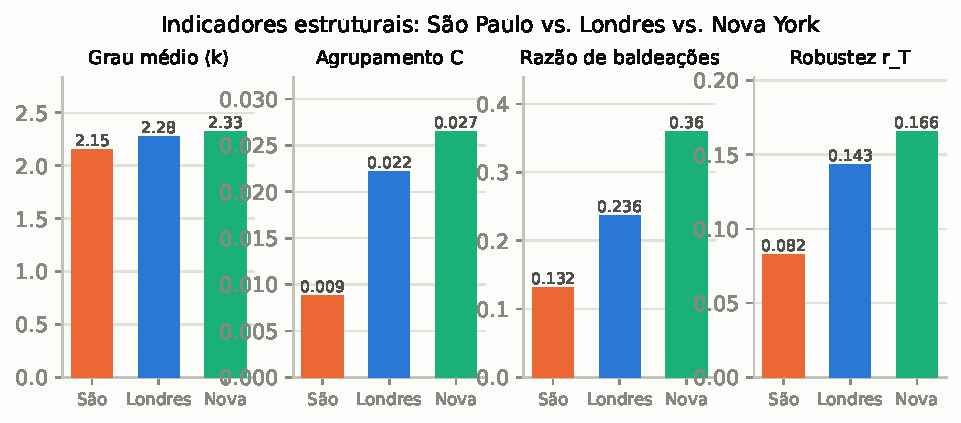
\includegraphics[width=\textwidth]{fig_ind3.pdf}
  \caption{Indicadores estruturais: São Paulo é consistentemente a mais esparsa.}
  \label{fig:ind3}
\end{figure}

\paragraph{Linha 6 e linhas em projeto.} O trecho atual da Linha 6 tem impacto
marginal ($+0{,}3\%$ de eficiência). A \emph{linha completa} (Brasilândia--São
Joaquim, $15{,}3$~km), com três novas baldeações (Água Branca, Higienópolis-
Mackenzie/L4, São Joaquim/L1)~\cite{agenciasp2026linha6}, eleva $E_{\mathrm{glob}}$
em $+0{,}62\%$. Modelando linhas em projeto pelas baldeações anunciadas
(Tabela~\ref{tab:propostas}), as extensões \emph{radiais} pouco mudam a
eficiência interna (seu ganho é de cobertura), enquanto a orbital \emph{20-Rosa}
produz o maior ganho ($+2{,}4\%$): o maior déficit de São Paulo é a
\emph{ausência de linhas circulares}, não a falta de raios. Custos são estimados
por obras de mesma natureza corrigidas (metrô subterrâneo $\approx$~R\$~$1{,}18$~bi/km,
da Linha 6; monotrilho $\approx$~R\$~$0{,}89$~bi/km, da Linha 17)~\cite{bndes2022linha6,metropoles2026expansao}.

\begin{table}[ht]
  \centering
  \caption{Linhas em projeto: extensão, custo estimado e papel na malha.}
  \label{tab:propostas}
  \small
  \begin{tabular}{@{}lrrl@{}}
    \toprule
    \textbf{Linha} & \textbf{km} & \textbf{Custo (R\$ bi)} & \textbf{Papel / ganho} \\
    \midrule
    6-Laranja (completa) & 15{,}3 & 18{,}1$^\dagger$ & Radial NO; $+0{,}6\%$ efic. \\
    20-Rosa              & 31{,}1 & $\approx$37 & \textbf{Orbital}; $+2{,}4\%$ efic. \\
    19-Celeste           & 17{,}6 & $\approx$21 & Radial (Guarulhos); cobertura \\
    22-Marrom            & 29{,}0 & $\approx$34 & Radial O (Cotia); cobertura \\
    16-Violeta           & 32{,}0 & $\approx$38 & Diagonal L--O; cobertura \\
    \bottomrule
  \end{tabular}

  {\footnotesize $^\dagger$ Valor real atualizado de 2024; demais são estimativas
  por km.}
\end{table}

% =====================================================================
\section{Análise e Discussão}
% =====================================================================

Os resultados convergem para um retrato coerente. A rede é dominada por dois
complexos (Luz, Brás) porque, sendo \emph{radial}, quase todo deslocamento entre
regiões atravessa o centro, o que os torna gargalos --- e a criticidade decorre
da \emph{posição} de ponte, não do grau (daí estações de grau $2$ com alta
intermediação). O diagnóstico estrutural é duplo: a malha não é livre de escala
(sem cauda longa) nem de mundo pequeno no espaço L ($\sigma<1$); é uma rede
espacial quase-planar, de baixo agrupamento e caminhos longos. A assimetria entre
falha e ataque é a face dinâmica dessa radialidade: com poucos ciclos
alternativos, remover $2\%$ das estações centrais fragmenta a rede, o que
recomenda redundância viária justamente no centro. A comparação internacional
reforça o quadro: entre São Paulo, Londres e Nova York, a paulistana é a menos
interconectada e a única fora do regime de mundo pequeno. Disso decorre a
principal recomendação: o maior ganho marginal de conectividade viria de
\emph{conexões circulares} (como a Linha 20-Rosa, $+2{,}4\%$) e não de novos raios
(Linha 6 completa, $+0{,}6\%$). \textbf{Limitações:} a análise é topológica (não
pondera demanda, capacidade ou tempo real); as simulações de linhas em projeto
usam baldeações anunciadas; e Nova York foi modelada por serviços, o que eleva
seus índices de redundância.

% =====================================================================
\section{Considerações Finais}
% =====================================================================

Modelamos a malha metroferroviária de São Paulo como grafo e a caracterizamos de
ponta a ponta: rede conexa, esparsa e radial, não livre de escala nem de mundo
pequeno no espaço L, dominada por Luz e Brás, frágil a ataques dirigidos e entre
os metrôs menos redundantes do mundo. A conclusão prospectiva é que o próximo
salto estrutural está nas linhas circulares, não em novos raios.

\textbf{Processo e equipe.} O trabalho seguiu um fluxo incremental --- curadoria
dos dados, construção do grafo (espaços L e P), implementação das métricas em
NetworkX, experimentos e redação --- mantido \emph{reprodutível} em repositório
público, o que evitou divergências entre texto, tabelas e figuras. As tarefas
foram divididas conforme a Tabela~\ref{tab:resp}, com o grafo serializado atuando
como ``contrato'' comum entre as frentes, integradas ao fim de cada etapa.
\textbf{Dificuldades e estratégias:} padronização de nomes de baldeação
(resolvida com nome canônico único por vértice); a configuração recente da Linha
6 (tratada separando trecho atual e completo); a escolha entre espaço L e P
(superada usando ambos); e a obtenção de coordenadas geográficas (ainda não
incorporadas, apontada como trabalho futuro, junto da rede multimodal e da
ponderação por tempo/demanda).

\begin{table}[ht]
  \centering
  \caption{Divisão de responsabilidades entre os integrantes.}
  \label{tab:resp}
  \small
  \begin{tabular}{@{}p{4.4cm}p{8.4cm}@{}}
    \toprule
    \textbf{Integrante} & \textbf{Responsabilidades principais} \\
    \midrule
    Vitor Eduardo Silva de Carvalho & Coordenação; coleta e curadoria dos dados;
      construção do grafo (espaços L e P). \\
    Diego Naoki Sato Hanashiro & Fundamentação teórica; métricas de centralidade e
      mundo pequeno em NetworkX. \\
    João Vitor Ribeiro Pereira & Robustez (falhas e ataques); comunidades; figuras
      e análise dos resultados. \\
    Joaquim Argolo Valente de Azambuja & Comparação internacional; redação e
      revisão no padrão SBC; integração final. \\
    \bottomrule
  \end{tabular}
\end{table}

\bibliographystyle{sbc}
\bibliography{refs}

\end{document}
